\chapter{Normalizing Flows}
\label{chapter:probmodel}

\section{Introduction}
The best known and studied probability distributions, which are analitically
manageable, are rarely expressive enough for real-world complex datasets, such
as images or signals. However, they have properties that make them amenable to
work with, for instance: tractable parameter estimation, closed-form likelihood
functions, and simple sampling procedures.

As described in the previous chapter, one way to obtain more expressive models is
to assume the existence of latent variables, leverage certain factorization
structures, and to use well-known distributions for the individual factors of the product that
constitutes the model's joint distribution. By using these structures and choosing
specific combinations of distributions (namely, conjugate prior-likelihood pairs),
these models are able to stay tractable - normally via bespoke estimation/inference/learning
algorithms.

%Structures are easily encoded by Probabilistic Graphical Models, which are a
%framework to easily express conditional independence assumptions and to specify
%complex probabilistic models.

Another approach to obtaining expressive probabilistic models is to apply
transformations to a simple distribution, and use the \emph{change of variables}
formula to compute probabilities in the transformed space. This is the basis
of \emph{normalizing flows}, an approach proposed by \citeauthor{shakir_nf} in \cite{shakir_nf},
and which has since evolved and developed into the basis of multiple state-of-the-art
techniques for density modelling and estimation (\autocite{Glow}, \autocite{real-nvp}, \autocite{bnaf19},
\autocite{NIPS2017_6828}).

\section{Change of Variables}
Given a random variable $\bm{z}$, with probability density function $f_Z$,
and a bijective and continuous function $g$, the probability density function $f_X$
of the random variable $\bm{x} = g(\bm{z})$ is given by
\begin{align}
    f_X(\bm{x}) &= f_Z(g^{-1}(\bm{x}))\Big|\det\Big(\frac{d}{d\bm{x}}g^{-1}(\bm{x})\Big)\Big|.
\end{align}

For this expression to be useful, some parts of it have to be easily computable:
\begin{itemize}
    \item $f_Z$ - the starting distribution's probability density function
        (also called \emph{base density}). It is assumed that there is a closed-form expression to
        compute this. In practice, this is typically one of the basic distributions
        (Gaussian, Uniform, etc.)
    \item $\det\Big(\frac{d}{d\bm{x}}g^{-1}(\bm{x})\Big)$ - the determinant  of the Jacobian
        matrix of $g^{-1}$ . For most transformations this is not \q{cheap} to compute.
        As will be shown, the main challenge o thef Normalizing Flows framework is
        to find transformations that are expressive enough, and for which the determinants
        of their Jacobian matrices are \q{cheap} to compute.
\end{itemize}

\section{Normalizing Flows}
Let us have $L$ transformations $h_\ell$, for $\ell = 0, 1, ... L$ that fulfill the two requirements listed
above. Let $\bm{z_\ell} = h_{\ell-1} \circ h_{\ell-2} \circ ... \circ h_0(\bm{z_0})$, where
$\bm{z_0}$ is sampledfrom $f_Z$, the base density. Furthermore, let $g$ be the composition of
the $L$ transformations. Applying the change of variables formula to
\begin{align}
    \bm{z_0} &\sim f_Z \\
    \bm{x} &= h_{L-1} \circ h_{L-2} \circ ... \circ h_0(\bm{z_0})
\end{align}
then
\begin{align}
    f_X(\bm{x}) &= f_Z(g^{-1}(\bm{x}))\Big|\det\Big(\frac{d}{d\bm{x}}g^{-1}(\bm{x})\Big)\Big| \\
                        &= f_Z(g^{-1}(\bm{x}))\prod_{\ell=0}^{L-1}\Big|\det\Big(\frac{d}{d\bm{z_{\ell+1}}}h_{\ell}^{-1}(\bm{z_{\ell+1}})\Big)\Big| \\
                        &= f_Z(g^{-1}(\bm{x}))\prod_{\ell=0}^{L-1}\Big|\det\Big(\frac{d}{d\bm{z_{\ell}}}h_{\ell}\Big(h_{\ell}^{-1}(\bm{z_{\ell+1}}\Big)\Big)\Big|^{-1} \label{eq:nflowderivation}
\end{align}

Replacing $h_{\ell}^{-1}(\bm{z_{\ell+1}}) = \bm{z_\ell}$ in \ref{eq:nflowderivation} leads to

\begin{align}
         f_X(\bm{x}) &= f_Z(g^{-1}(\bm{x}))\prod_{\ell=0}^{L-1}\Big|\det\Big(\frac{d}{d\bm{z_{\ell}}}h_{\ell}\Big(\bm{z_\ell})\Big)\Big)\Big|^{-1};
\end{align} taking the logarithm,
\begin{align}
    \log f_X(\bm{x}) &= \log f_Z(g^{-1}(\bm{x})) - \sum_{\ell=0}^{L-1} \log \Big|\det\Big(\frac{d}{d\bm{z_{\ell}}}h_{\ell}(\bm{z_\ell})\Big) \Big| \label{eq:nflowsfinal}
\end{align}

Depending on the task, one might prefer to replace the second term in \ref{eq:nflowsfinal}
with a sum of log-absolute-determinants of the Jacobians of the inverse transformations.
This switch would imply replacing the minus sign before the sum with a plus sign:
\begin{align}
    \log f_X(\bm{x}) &= \log f_Z(g^{-1}(\bm{x})) + \sum_{\ell=0}^{L-1} \log \Big|\det\Big(\frac{d}{d\bm{z_{\ell+1}}}h_{\ell}^{-1}(\bm{z_{\ell+1}})\Big) \Big|
\end{align}

With this expression, gradient-based MLE becomes feasible. Moreover, sampling
from the resulting distribution is simply achieved by sampling from the base
distribution and applying the chain of transformations. Because of this, Normalizing
Flows lend themselves to be used as flexible variational posteriors, in Variational
Inference settings.

\section{Examples of transformations}
\subsection{Affine Transformation}
An affine transformation is arguably the simplest choice. This transformation can
stretch, sheer, shrink, rotate, and translate the space. It is simply achieved
by the multiplication by a matrix $A$ and summation of a bias vector $\bm{b}$:
\begin{align}
    \bm{z} &\sim p(\bm{z}) \\
    \bm{x} &= A\bm{z} + \bm{b}
\end{align}
The determinant of the Jacobian of this transformation is simply the determinant
of the matrix $A$. However, in general, computing the determinant of a $N \times N$
matrix has $\mathcal{O}(N^3)$. For that reason, it is common to use matrices with
a certain structure which makes their determinants easier to compute. For
instance, if $A$ is triangular, its determinant is simply the product of its
diagonal's elements. The downside of using matrices that are constrained to
a certain structure is that they correspond to less flexible transformations.

It is possible, however, to design affine transformations whose Jacobian determinants
are of $\mathcal{O}(N)$ complexity and that are more expressive than simple
triangular matrices. In \autocite{Glow}, one such transformation is proposed. It
constrains the matrix $A$ to be decomposable as $A = PL\big(U + diag(\bm{s})\big)$,
where $diag(\bm{s})$ is a diagonal matrix whose diagonal's elements are
the values of vector $\bm{s}$. The following additional constrains are in place:
\begin{itemize}
    \item $P$ is a permutation matrix
    \item $L$ is a lower triangular matrix, with ones in the diagonal
    \item $U$ is an upper triangular matrix, with zeros in the diagonal
\end{itemize}
Given these constraints, the determinant of the matrix $A$ is simply the product
of the elements of $\bm{s}$.

\begin{figure}[!htb]
  \begin{subfigmatrix}{2}
    \subfigure[]{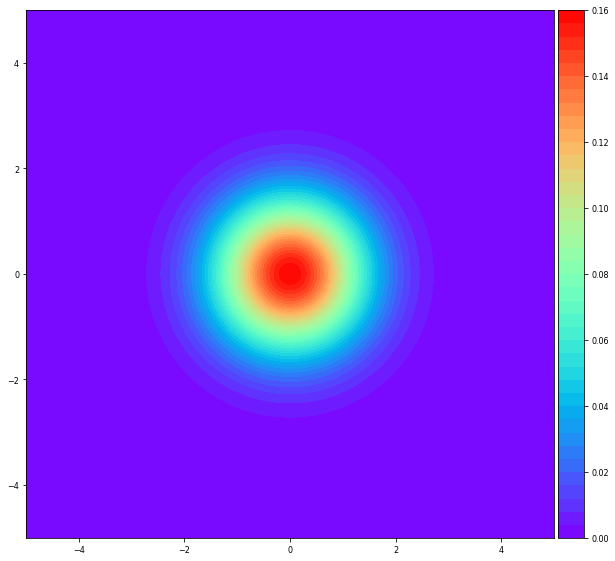
\includegraphics[width=0.49\linewidth]{figures/base_distribution.png}}
    \subfigure[]{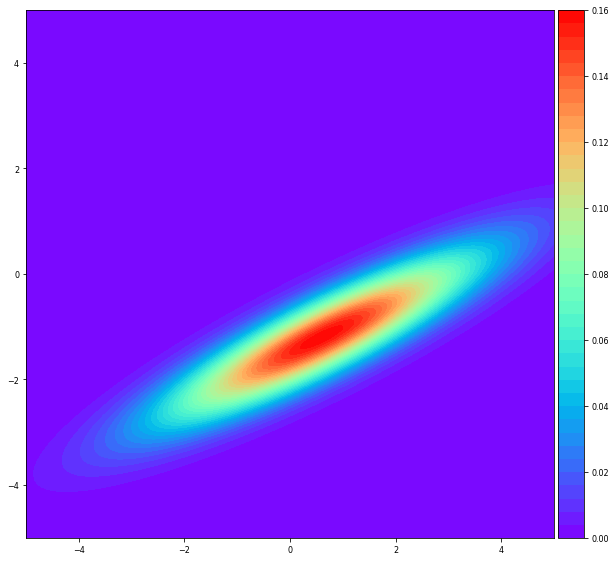
\includegraphics[width=0.49\linewidth]{figures/affine_transform.png}}
  \end{subfigmatrix}
    \caption{(a) Density of a Gaussian distribution with $\mu = [0, 0]$ and $\Sigma = I$
    (b) Density of the distribution that results from applying some affine transformation to
    the Gaussian distribution in (a)
    }
  \label{fig:affine}
\end{figure}

\subsection{PReLU Transformation}
Intuitively, introducing non-linearity endows normalizing flows with more flexibility to
represent complex distributions. This can be done in similar fashion to the
activation functions of neural networks. One example of that, is the parameterized
rectified linear unit transformation. It is defined in the following manner, for
a $d$-dimensional input:
\begin{align}
f_i(z_i) =
    \begin{cases}
        z_i,              & \text{if } z_i\geq 0\\
        \alpha z_i,       & \text{otherwise}
    \end{cases} \\
f(\bm{z}) = [f_0(z_0), f_1(z_1), ..., f_d(z_d)]
\end{align}
Note that in order for the transformation to be invertible, it is necessary
that $\alpha > 0$.

Let us define an auxiliary function $j(.)$ as
\begin{align}
j(z_i) =
    \begin{cases}
       1 ,              & \text{if } z_i \geq 0\\
       \alpha ,       & \text{otherwise}
    \end{cases}
\end{align}
It's trivial to see that the Jacobian of the transformation is a diagonal
matrix, whose diagonal elements are $j(z_i)$:
\begin{align}
  J(f(z)) =
  \begin{bmatrix}
      j(z_0) & & & \\
      & j(z_1) & & \\
      & & \ddots & \\
      & & & j(z_d)
  \end{bmatrix}
\end{align}
With that, it is easy to arrive at the log-absolute-determinant of this transformation's
Jacobian, which is given by $\sum_{i=0}^d \log \Big| j(z_i) \Big|$

\begin{figure}[!htb]
  \begin{subfigmatrix}{2}
    \subfigure[]{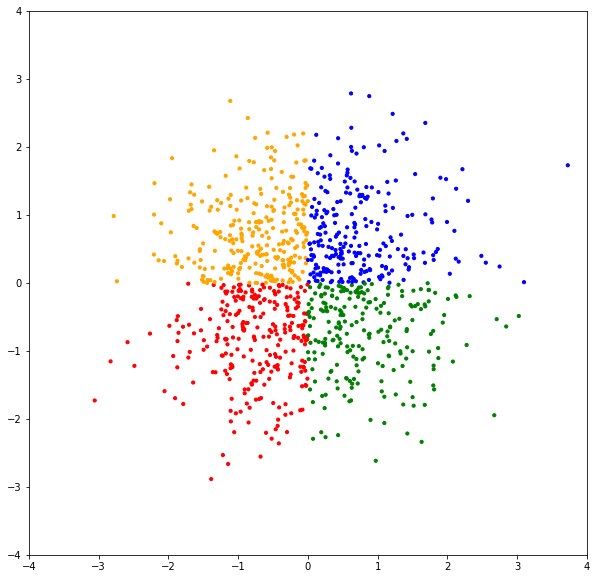
\includegraphics[width=0.49\linewidth]{figures/gaussian_in_quadrants.png}}
    \subfigure[]{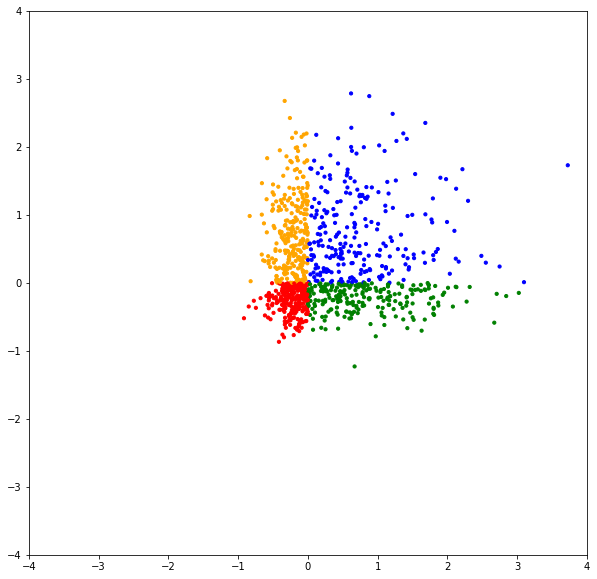
\includegraphics[width=0.49\linewidth]{figures/prelu_in_quadrants.png}}
  \end{subfigmatrix}
    \caption{(a) Samples from of a Gaussian distribution with $\mu = [0, 0]$ and $\Sigma = I$.
    The samples are colored according to the quadrant they belong to. (b) Samples from the
    distribuion in a) transformed by a PReLU transformation.}
  \label{fig:prelu}
\end{figure}

\begin{figure}[!htb]
  \begin{subfigmatrix}{3}
    \subfigure[]{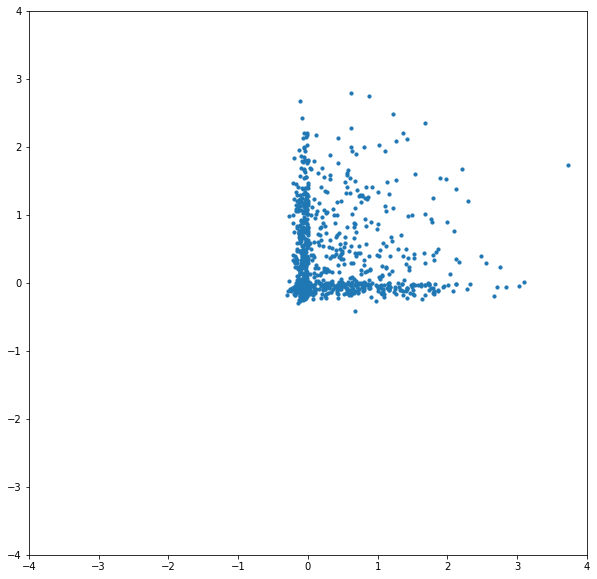
\includegraphics[width=0.31\linewidth]{figures/prelu_0_1.png}}
    \subfigure[]{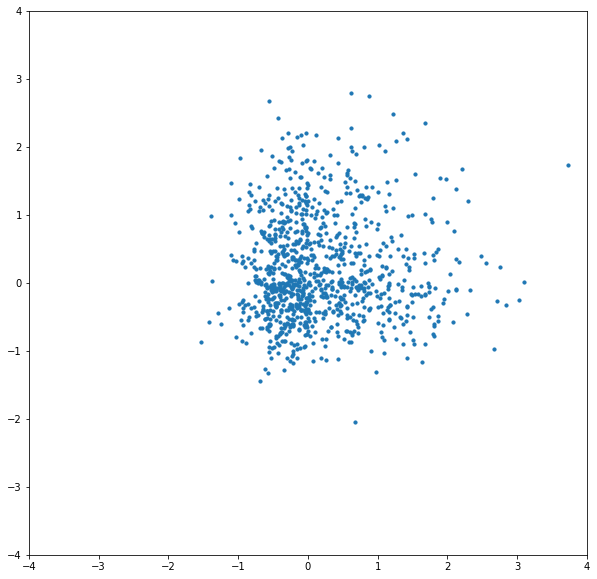
\includegraphics[width=0.31\linewidth]{figures/prelu_0_5.png}}
    \subfigure[]{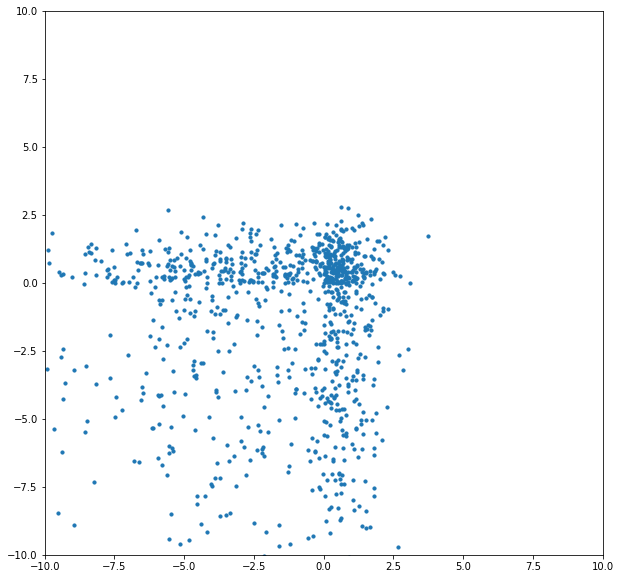
\includegraphics[width=0.31\linewidth]{figures/prelu_5.png}}
  \end{subfigmatrix}
    \caption{Samples from a Gaussian with $\mu = [0, 0]$ and $\Sigma = I$, transformed
    by PReLU transformations with different $\alpha$ parameters. (a) $\alpha = 0.1$
    (b) $\alpha = 0.5$ (c) $\alpha = 5$}
  \label{fig:prelu}
\end{figure}

\subsection{Batch-Normalization Transformation}
In \cite{real-nvp}, the authors propose a batch-normalization transformation, similar to
the well-known batch-normalization layer normally used in neural networks. This
transform simply applies a rescaling, given the batch mean $\tilde\mu$ and variance
${\tilde\sigma}^2$:
\begin{align}
    f(z) = \frac{z - \tilde\mu}{\sqrt{{\tilde\sigma}^2 + \epsilon}},
\end{align} where $\epsilon \ll 1$ is a term used to ensure that there never is
a division by zero. This transformation's Jacobian is trivial: 
\begin{align}
    \prod_i \frac{1}{\sqrt{{\tilde\sigma}_i^2 + \epsilon}}.
\end{align}

\subsection{Affine Coupling Transformation}
As mentioned previously, one of the active research challenges within the
normalizing flows framework is the search and design of transformations that
are expressive and whose Jacobians are not computationally heavy. One brilliant
example of such transformations was proposed by \citeauthor{real-nvp} in
\cite{real-nvp}, and is called affine coupling layer.

This transformation is characterized by two \textbf{arbitrary} functions $s(.)$ and
$t(.)$, as well as a mask that splits an input $\bm{z}$ of dimension $D$ into
two parts, $\bm{z_1}$ and $\bm{z_2}$. In practice, $s(.)$ and $t(.)$ are
neural networks, whose parameters will be optimized so as to make the transformation
approximate the desired output distribution. The outputs of $s(.)$ and $t(.)$
need to have the same dimension as $\bm{z_1}$. This should be taken into account when
designing the mask and the functions $s(.)$ and $t(.)$. It is defined as:

\begin{align}
    \bm{x_1} &= \bm{z_1} \odot \exp\big(s(\bm{z_2})\big) + t(\bm{z_2}) \\
    \bm{x_2} &= \bm{z_2}
\end{align}

To see why this transformation is suitable to being used within the framework
of normalizing flows, let us derive its Jacobian.
\begin{itemize}
    \item $\frac{\partial \bm{x_2}}{\partial \bm{z_2}} = I$ is trivial, because $\bm{x_2} = \bm{z_2}$.
    \item $\frac{\partial \bm{x_2}}{\partial \bm{z_1}}$ is a matrix of zeros, because $\bm{x_2}$ does not depend on $\bm{z_1}$.
    \item $\frac{\partial \bm{x_1}}{\partial \bm{z_1}}$ is a diagonal matrix,
        whose diagonal is simply given by $\exp\big(s(\bm{z_2})\big)$, since those values are
        constant w.r.t $\bm{z_1}$ and they are multiplying each element of $\bm{z_1}$.
    \item $\frac{\partial \bm{x_1}}{\partial \bm{z_2}}$ is not needed for our purposes,
        as will become clear ahead.
\end{itemize}

Writing the above in matrix form:
%\[
%\begin{bmatrix}
%  \mbox{\huge$\frac{\partial \bm{x_1}}{\partial \bm{z_1}}$} & \mbox{\huge$\frac{\partial \bm{x_1}}{\partial \bm{z_2}}$} \\
%  \mbox{\huge$\frac{\partial \bm{x_2}}{\partial \bm{z_1}}$} & \mbox{\huge$\frac{\partial \bm{x_2}}{\partial \bm{z_2}}$} \\
%\end{bmatrix}
%\]


\begin{align}
    J_{f(z)} &=
        \begin{tikzpicture}[decoration=brace, baseline=-\the\dimexpr\fontdimen22\textfont2\relax ]
            \matrix (m) [matrix of math nodes,left delimiter=[,right delimiter={]}, ampersand replacement=\&] {
                \mbox{\Large$\frac{\partial \bm{x_1}}{\partial \bm{z_1}}$} \& \mbox{\Large$\frac{\partial \bm{x_1}}{\partial \bm{z_2}}$} \\
                \mbox{\Large$\frac{\partial \bm{x_2}}{\partial \bm{z_1}}$} \& \mbox{\Large$\frac{\partial \bm{x_2}}{\partial \bm{z_2}}$} \\
            };
%            \draw[decorate,transform canvas={xshift=-1.5em},thick] ($ (m-1-1.south west) +(0,3pt) $)
%                -- node[left=2pt] {$\frac{\partial \bm{x_1}}{\partial (.)}$} ($ (m-1-1.north west) -(0,3pt) $);
%            \draw[decorate,transform canvas={xshift=-1.5em},thick] ($ (m-2-1.south west) +(0,3pt) $)
%                -- node[left=2pt] {$\frac{\partial \bm{x_2}}{\partial (.)}$} ($ (m-2-1.north west) -(0,3pt) $);
%            \draw[decorate,transform canvas={yshift=0.5em},thick] ($ (m-1-1.north west) +(2pt,0) $)
%                -- node[above=2pt] {$\frac{\partial (.)}{\partial \bm{z_1}}$} ($ (m-1-1.north east) -(2pt,0) $);
%            \draw[decorate,transform canvas={yshift=0.5em},thick] ($ (m-1-2.north west) +(2pt,0) $)
%                -- node[above=2pt] {$\frac{\partial (.)}{\partial \bm{z_2}}$} ($ (m-1-2.north east) +(2pt,0) $);
        \end{tikzpicture} \\
    &=
        \begin{tikzpicture}[decoration=brace, baseline=-\the\dimexpr\fontdimen22\textfont2\relax ]
            \matrix (m) [matrix of math nodes,left delimiter=[,right delimiter={]}, ampersand replacement=\&] {
                diag\Big(\exp\big(s(\bm{z_2})\big)\Big) \& \mbox{\Large$\frac{\partial \bm{x_1}}{\partial \bm{z_2}}$} \\
                \mbox{\Large$\bm{0}$} \& \mbox{\Large$I$} \\
            };
        \end{tikzpicture}
\end{align} shows that the Jacobian matrix is triangular. Its determinant - the
only thing we need, in fact - is therefore easy to compute: it is simply the
product of the diagonal elements. Moreover, part of the diagonal is simply
composed of ones. The determinant, and the log-absolute-determinant become
\begin{align}
    det\big(J_{f(z)}\big) &= \prod_i \exp\big(s(\bm{z_2}^{(i)})\big) \\
    \log \Big|det\big(J_{f(z)}\big)\Big| &= \sum_i s(\bm{z_2}^{(i)}),
\end{align} where $\bm{z_2^{(i)}}$ is the $i$-th element of $\bm{z_2}$.
Since a single affine coupling layer does not transform all of the elements in
$\bm{z}$, in practice several layers are composed, and each layer's mask is changed
so as to make all dimensions affect each other. This can be done, for instance, with
a checkerboard pattern, which alternates for each layer. In the case of image inputs,
the masks can operate at the channel level.

\section{Fitting Normalizing Flows}

Generally speaking, normalizing flows can be used in one of two scenarios:
(direct) density estimation, where the goal is to optimize the parameters
so as to make the model approximate the distribution of some observed set of data;
in a variational inference scenario, as way of having a flexible variational
posterior (i.e. $q(\bm{z})$ in the terminology used in the previous chapter). The
second scenario is out of the scope of this work.

The task of density estimation with normalizing flows reduces to finding the
optimal parameters of a parametric model. As mentioned in section \ref{section:map-mle},
there are two ways to go about estimating the parameters of a parametric model,
given data: MLE and MAP. In the case of normalizing flows, MLE is the usual
approach\footnote{In theory it is possible to place a prior on the normalizing
flow's parameters and do MAP estimation. To accomplish this, similar strategies
to those used in Bayesian Neural Networks would have to be used.}. To fit a normalizing
flow via MLE, a gradient based optimizer is used to minimize
$\hat{\mathcal{L}}(\bm\theta) = - \mathbb{E}[\log p(\bm{x}|\bm\theta)]$
